\documentclass[8pt,a4paper]{article} % Compila con lualatex o xelatex

% --- Layout & links ---
\usepackage[margin=1.5in]{geometry}
\usepackage[hidelinks]{hyperref}

% --- Fuentes (texto y matemáticas) ---
\usepackage{newtxmath}
\usepackage{fontspec}
% \setmainfont{EB Garamond}[
%   UprightFont = * Medium,
%   ItalicFont = * Medium Italic,
%   BoldFont = * SemiBold,
%   BoldItalicFont = * SemiBold Italic
% ]
\setmainfont{EB Garamond}[
  UprightFont = * Regular,
  ItalicFont = * Italic,
  BoldFont = * SemiBold,
  BoldItalicFont = * SemiBold Italic
]

% --- Secciones y subsecciones ---
\usepackage{titlesec}
\newfontface\garamondbold{EB Garamond SemiBold}
\newfontface\garamondbolditalic{EB Garamond SemiBold Italic}
\titleformat{\section}
  {\garamondbold\Large}{\thesection}{1em}{}
\titleformat{\subsection}
  {\garamondbold\Large}{\thesubsection}{1em}{}

% --- Encabezado con nombre de la sección ---
\usepackage{fancyhdr}
\pagestyle{fancy}
\fancyhf{}
\fancyhead[L]{\small\leftmark}
\fancyhead[R]{\small\thepage}
\renewcommand{\headrulewidth}{0.0pt}

% --- Espaciado ---
\usepackage{setspace}

% --- Otros paquetes útiles ---
\usepackage{tocloft}  % Para personalizar la tabla de contenidos
\usepackage{xcolor}   % Para colores en el código
\usepackage{booktabs} % Para tablas bonitas
\usepackage{graphicx} % Para las graficas
\graphicspath{{../../../../visualizations/figuras/}}


% --- Código fuente ---
\usepackage{listings}
\lstset{
  basicstyle=\ttfamily\small,
  backgroundcolor=\color{gray!10},
  frame=single,
  breaklines=true
}


\usepackage{chngcntr}       % in preamble
\numberwithin{figure}{subsection}


\usepackage{lipsum}

\begin{document}

% --- Portada ---
\begin{titlepage}
  \centering
  \vspace*{4cm}
  {\Huge\bfseries CMAT\par}
  \vspace{2cm}
  {\Large Author Name\par}
  \vspace{1cm}
  {\large Universidad de las Américas Puebla\par}
  \vfill
  {\large \today\par}
\end{titlepage}

% --- Abstract ---
\begin{abstract}
This document provides a template for reports in the "AI in Financial Services" course, using EB Garamond for prose and Libertinus Math for formulas. It includes a cover page, abstract, table of contents, and sample sections for math and text. Additional content demonstrates tables, code, and references.
\end{abstract}

% --- Tabla de contenidos ---
\tableofcontents
\thispagestyle{empty}
\newpage

% --- Inicio del documento ---
\section{Overview}
This document is a minimal example using EB Garamond for prose and libertinust1math for formulas.
Links like \href{https://example.com}{this one} are active.


\newpage
\section{What is CMAT?}
Centro de Matematicas, (Math Center), is a place where students go to take assesorias.



\newpage
\section{Exploratory Data Analysis}
\lipsum[1]

\subsection{How many people went to CMAT?}
\lipsum[1]

\begin{figure}[h]
    \centering
    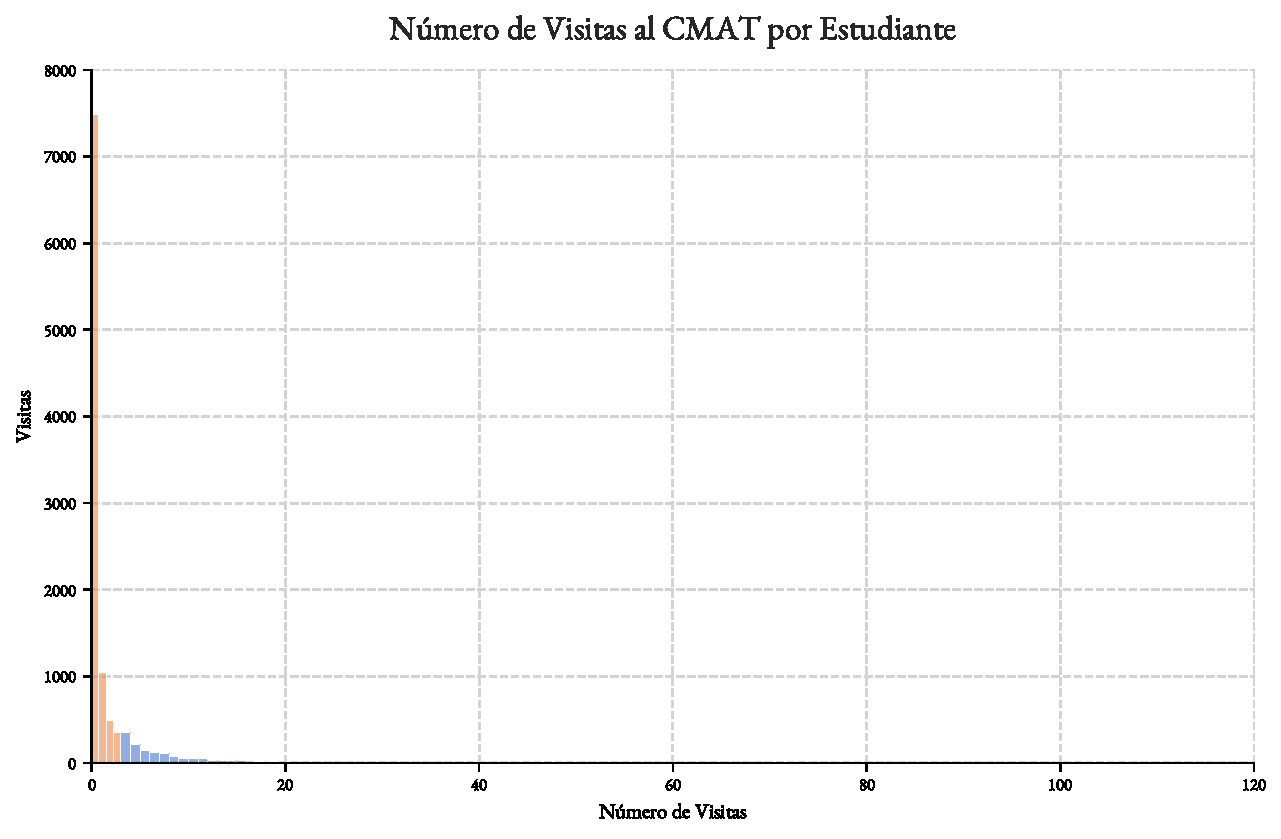
\includegraphics[width=0.7\textwidth,page=1]{03_01.pdf}
    \caption{PDF imported as image}
\end{figure}

\begin{figure}[h]
    \centering
    
\includegraphics[width=0.7\textwidth,page=1]{03_02.pdf}
    \caption{PDF imported as image}
\end{figure}



\newpage
\section{Are they better?}
\lipsum[1]

\subsection{How do we quantify that?}
\lipsum[1]

\subsection{Then, how do we compare it?}
Sup: With their califications.


\newpage
\section{Califications}
\lipsum[1]


\subsection{Why are there missing values?}
Students have the option to do not recieve calification.

Sup: Students dont want to recieve calification when they will not pass the course.

\subsection{Imputation of missing values}
\lipsum[1]


\subsection{The califications are relatable?}
\lipsum[1]

\begin{figure}[h]
    \centering
    
\includegraphics[width=0.7\textwidth,page=1]{05_01.pdf}
    \caption{PDF imported as image}
\end{figure}

Special cases

\begin{figure}[h]
    \centering
    
\includegraphics[width=0.5\textwidth,page=1]{05_03.pdf}
    \caption{PDF imported as image}
\end{figure}
\lipsum[1]

\begin{figure}[h]
    \centering
    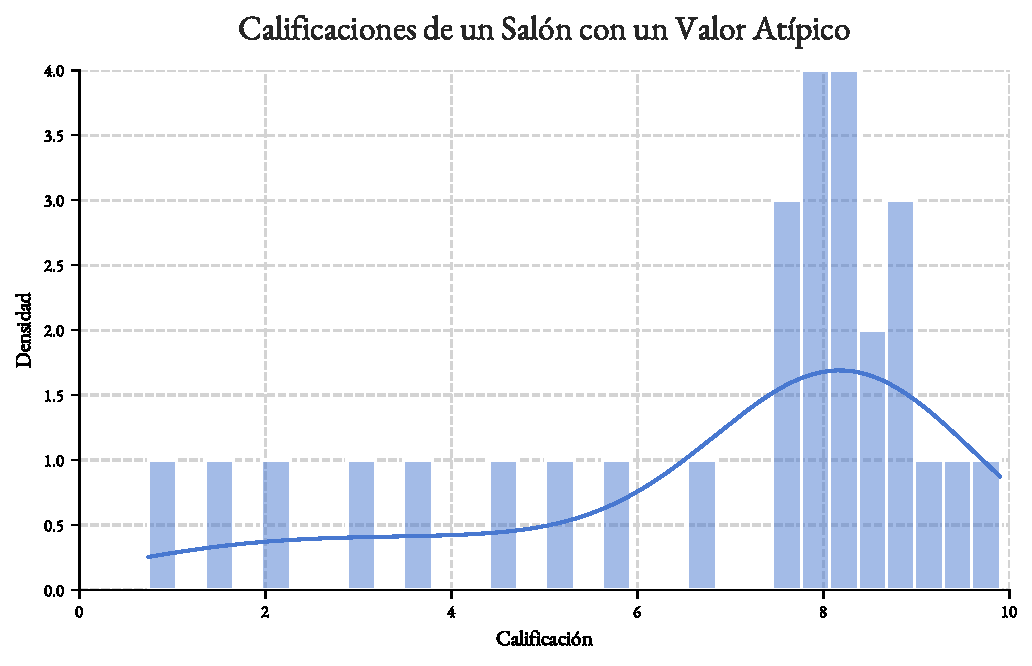
\includegraphics[width=0.5\textwidth,page=1]{05_04.pdf}
    \caption{PDF imported as image}
\end{figure}
\lipsum[1]

\begin{figure}[h]
    \centering
    
\includegraphics[width=0.7\textwidth,page=1]{05_05.pdf}
    \caption{PDF imported as image}
\end{figure}
\lipsum[1]

\begin{figure}[h]
    \centering
    
\includegraphics[width=0.7\textwidth,page=1]{05_06.pdf}
    \caption{PDF imported as image}
\end{figure}
\lipsum[1]

\begin{figure}[h]
    \centering
    
\includegraphics[width=0.7\textwidth,page=1]{05_07.pdf}
    \caption{PDF imported as image}
\end{figure}
\lipsum[1]

\subsection{How does the teachers calificate their students?}
\lipsum[1]

\begin{figure}[h]
    \centering
    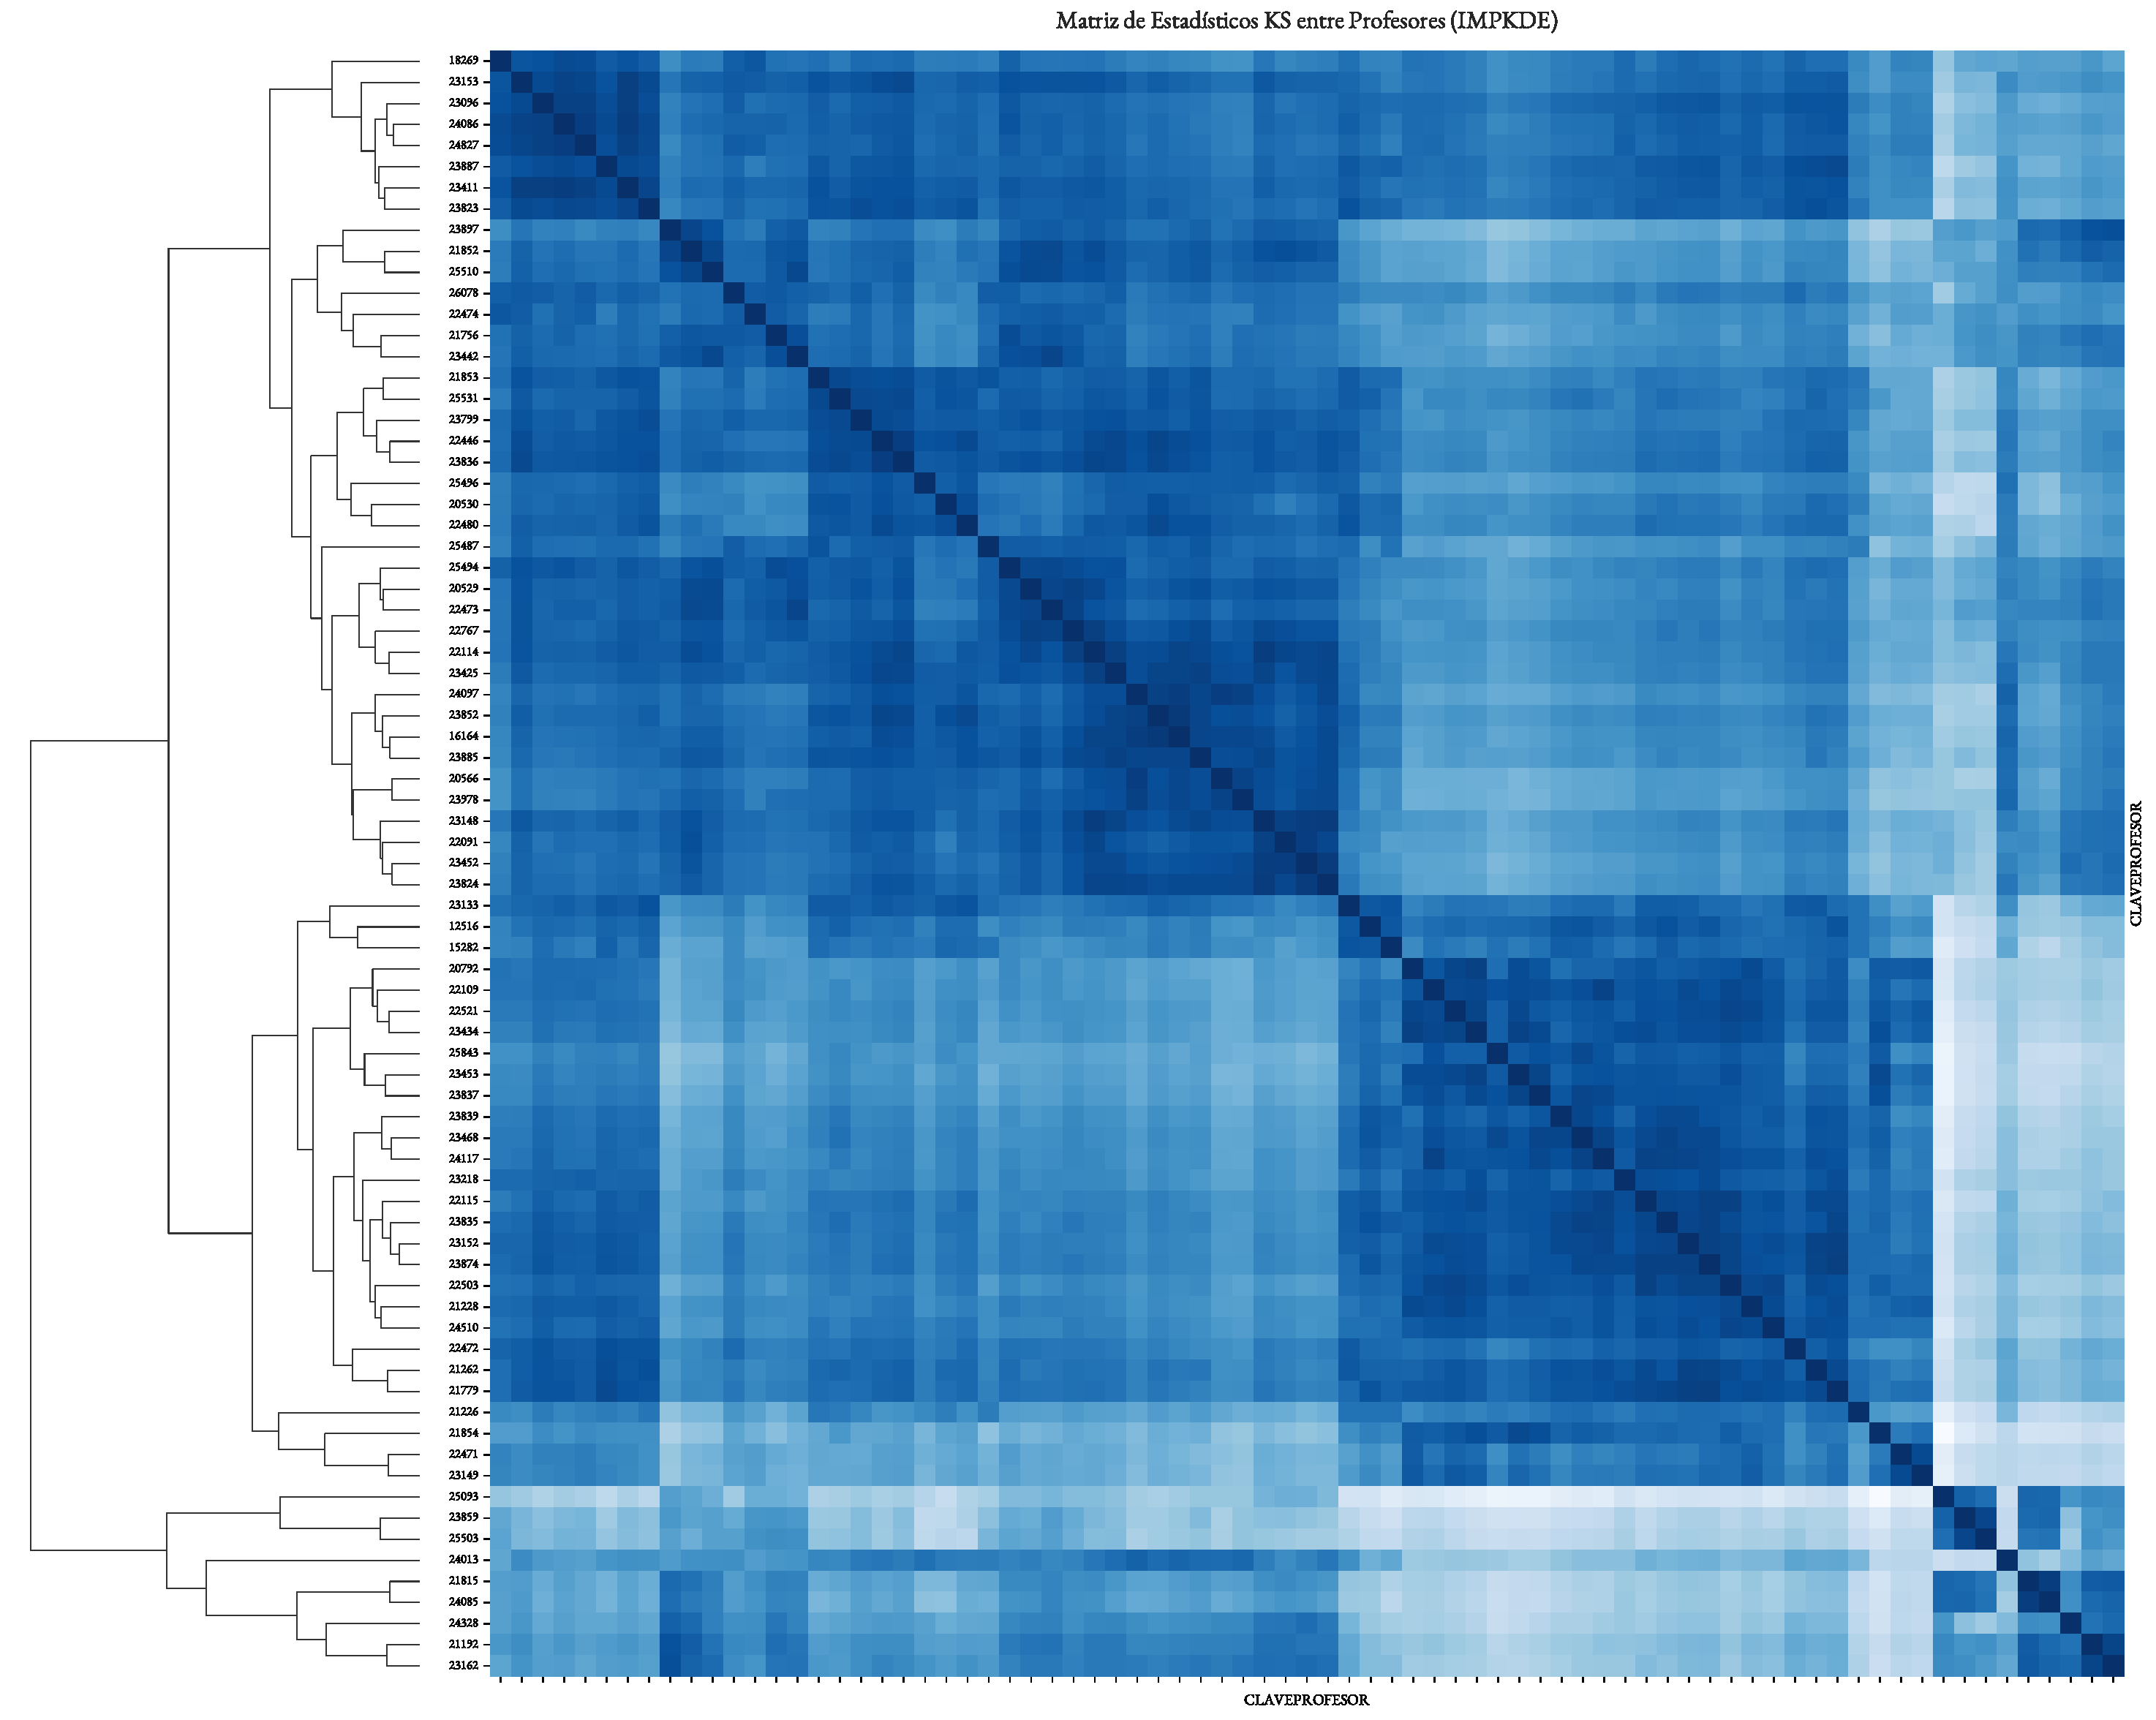
\includegraphics[width=0.7\textwidth,page=1]{05_08.pdf}
    \caption{PDF imported as image}
\end{figure}
\lipsum[1]

\begin{figure}[h]
    \centering
    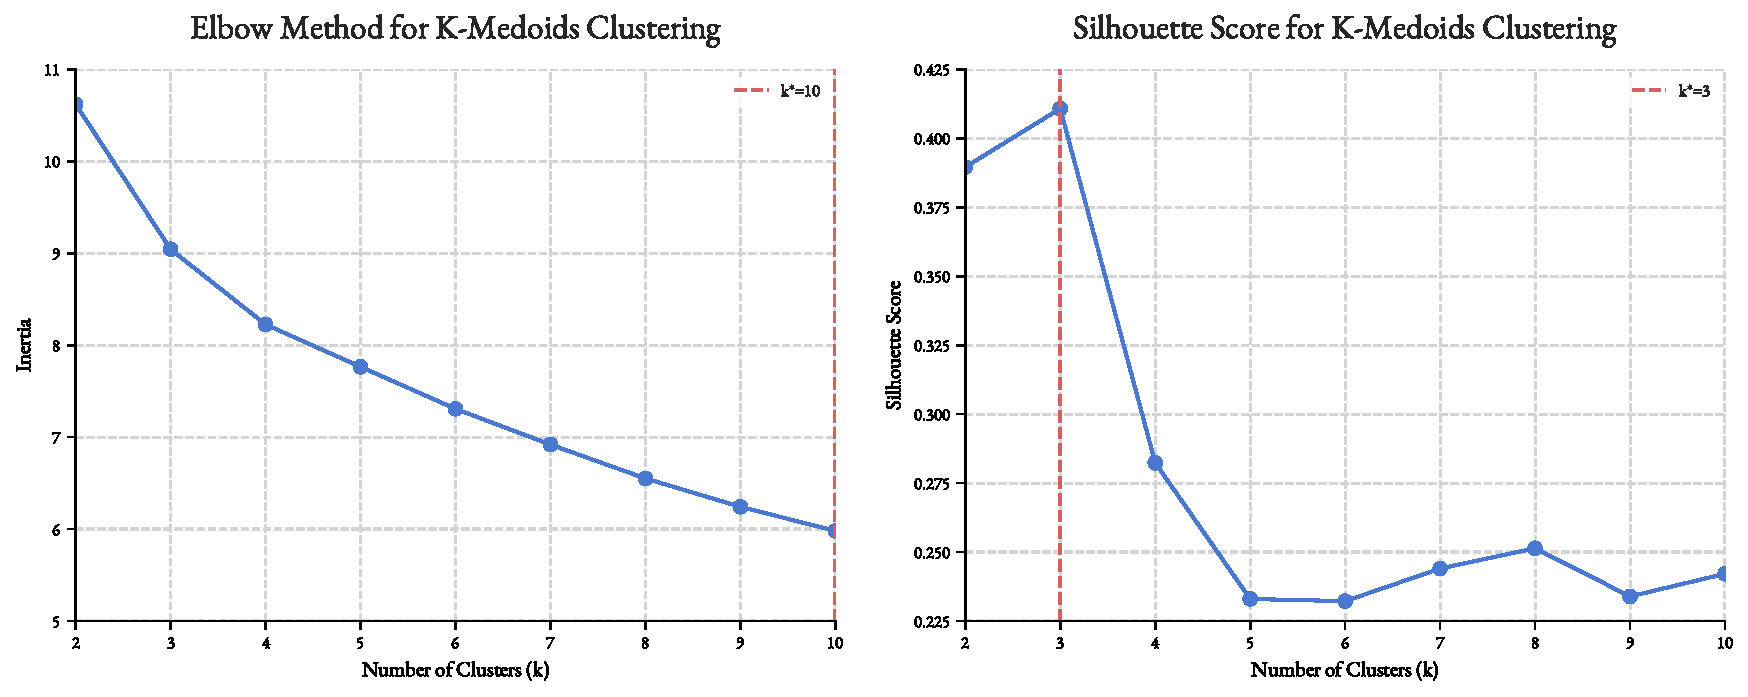
\includegraphics[width=0.7\textwidth,page=1]{05_09.pdf}
    \caption{PDF imported as image}
\end{figure}
\lipsum[1]

\begin{figure}[h]
    \centering
    
\includegraphics[width=0.7\textwidth,page=1]{05_10_0.pdf}
    \caption{PDF imported as image}
\end{figure}
\lipsum[1]

\begin{figure}[h]
    \centering
    
\includegraphics[width=0.7\textwidth,page=1]{05_10_1.pdf}
    \caption{PDF imported as image}
\end{figure}
\lipsum[1]

\begin{figure}[h]
    \centering
    
\includegraphics[width=0.7\textwidth,page=1]{05_10_2.pdf}
    \caption{PDF imported as image}
\end{figure}
\lipsum[1]



\begin{figure}[h]
    \centering
    
\includegraphics[width=0.7\textwidth,page=1]{05_11_0.pdf}
    \caption{PDF imported as image}
\end{figure}
\lipsum[1]

\begin{figure}[h]
    \centering
    
\includegraphics[width=0.7\textwidth,page=1]{05_11_1.pdf}
    \caption{PDF imported as image}
\end{figure}
\lipsum[1]

\begin{figure}[h]
    \centering
    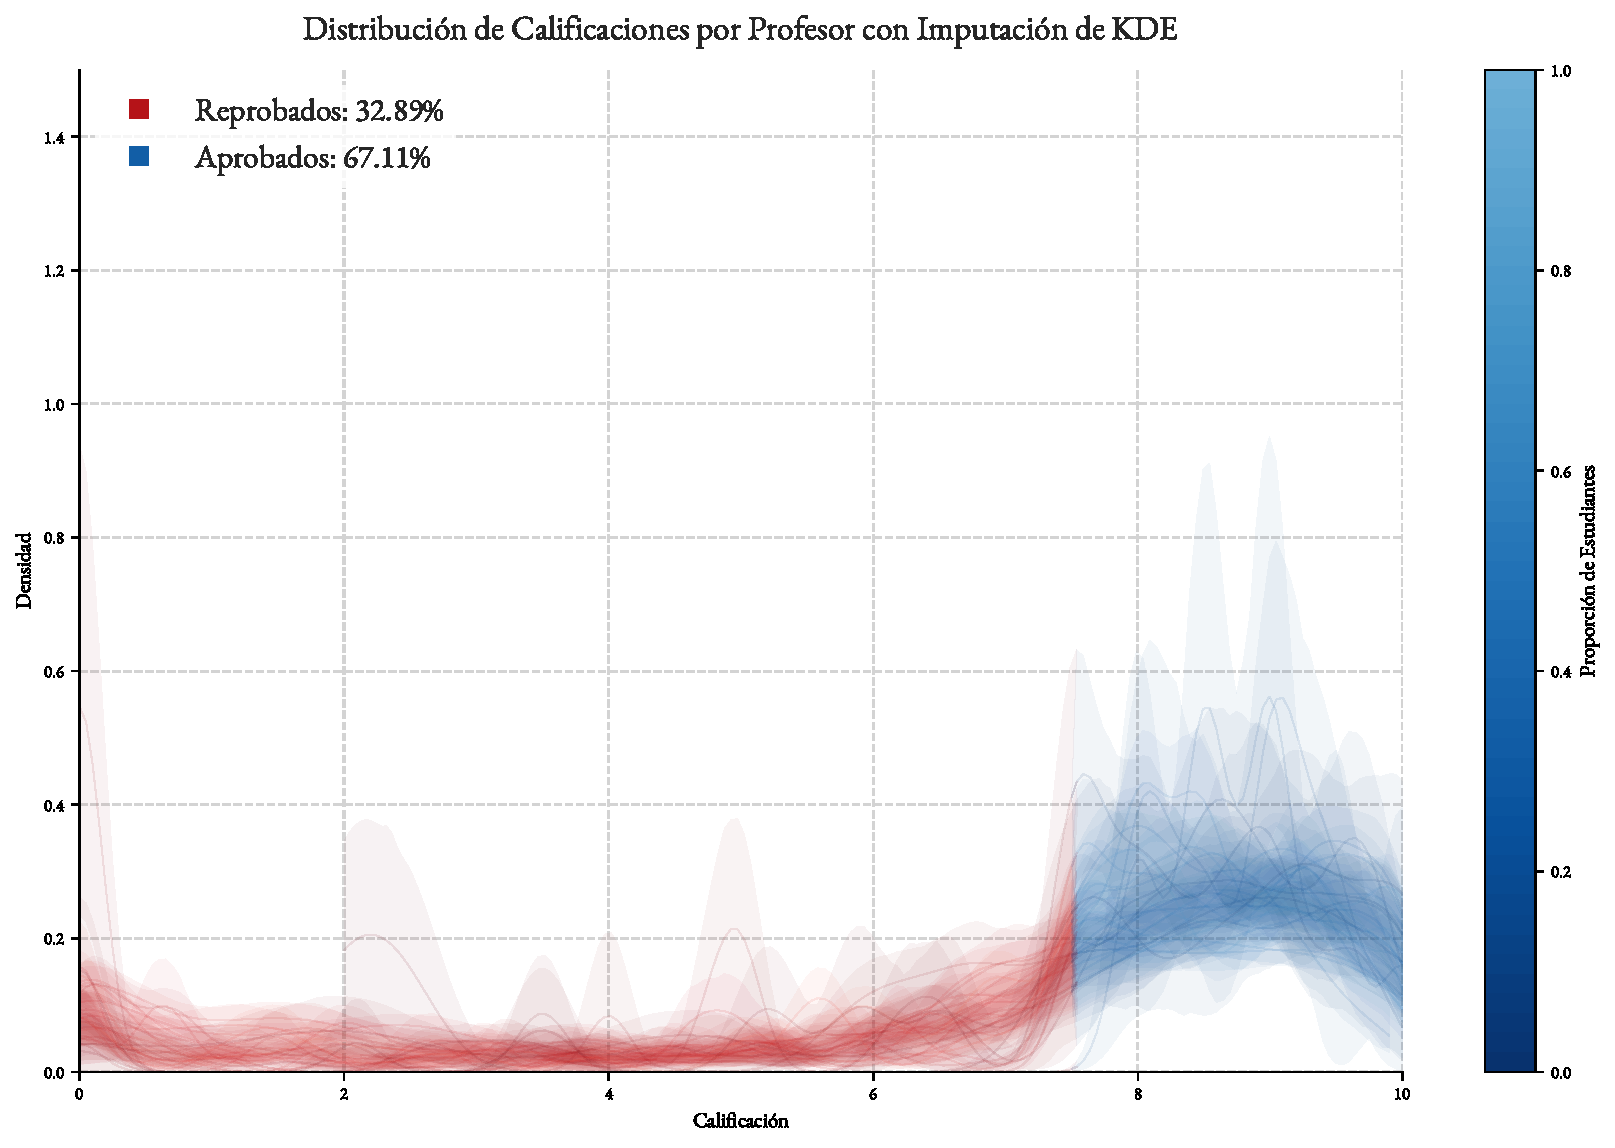
\includegraphics[width=0.7\textwidth,page=1]{05_11_2.pdf}
    \caption{PDF imported as image}
\end{figure}
\lipsum[1]


Answer: There are 3 ways of califications



\newpage
\section{Which is the best way to estandarize?}
\lipsum[1]

\subsection{The calificotions depends on the teacher}
\lipsum[1]

\subsection{The califications depend on the teacher at time $t$}
\lipsum[1]

\begin{figure}[h]
    \centering
    
\includegraphics[width=0.7\textwidth,page=1]{06_00.pdf}
    \caption{PDF imported as image}
\end{figure}
\lipsum[1]


\subsection{Then, by salon}

We standarize by classroom.

Hooray! We got it.

\newpage
\section{Analysis by calification}
\lipsum[1]

\begin{figure}[h]
    \centering
    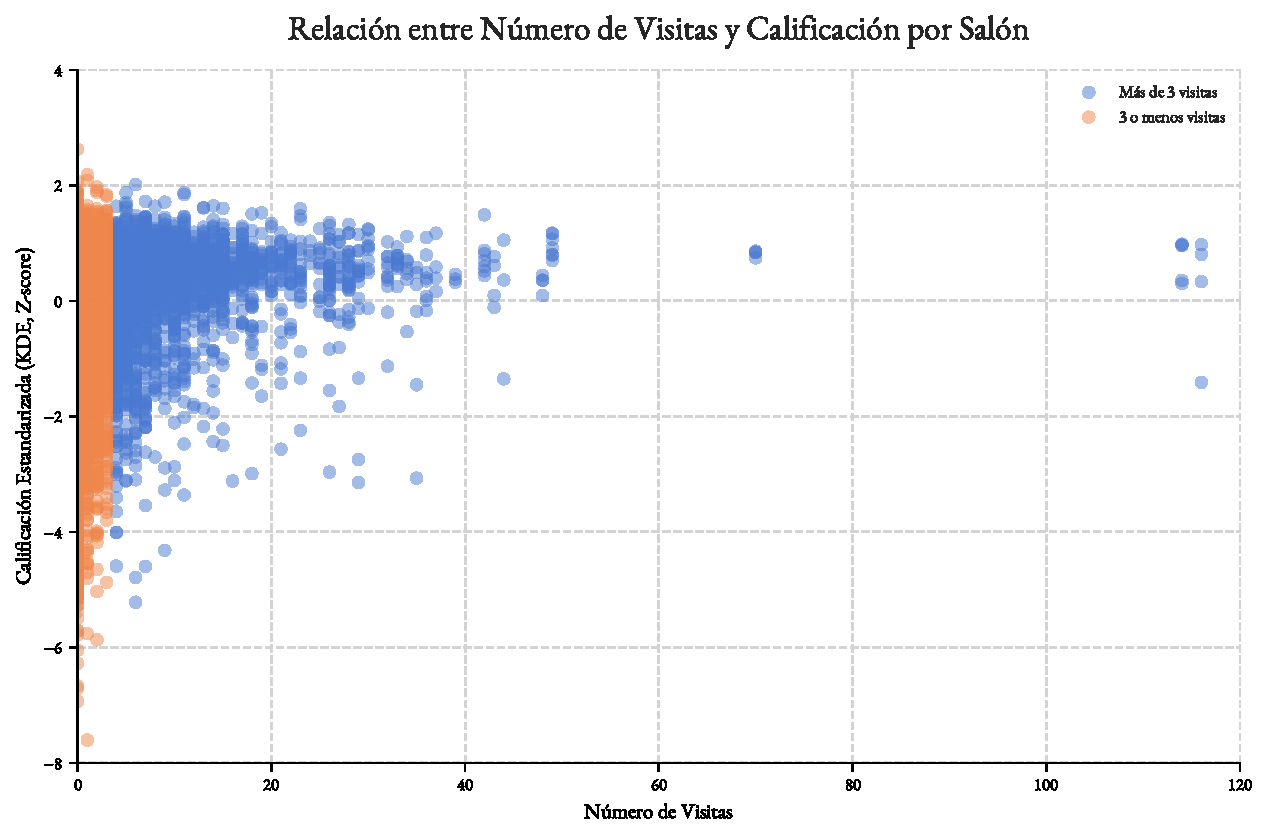
\includegraphics[width=0.7\textwidth,page=1]{07_00.pdf}
    \caption{PDF imported as image}
\end{figure}
\lipsum[1]

\subsection{Difference of means}
\lipsum[1]

\begin{figure}[h]
    \centering
    
\includegraphics[width=0.7\textwidth,page=1]{07_01.pdf}
    \caption{PDF imported as image}
\end{figure}
\lipsum[1]

\subsection{Confidence Intervals}
\lipsum[1]

\subsection{Robust tests}
\lipsum[1]

\begin{figure}[h]
    \centering
    
\includegraphics[width=0.7\textwidth,page=1]{07_02.pdf}
    \caption{PDF imported as image}
\end{figure}
\lipsum[1]

\subsection{Confidence intervals}
\lipsum[1]

\subsection{Interpretation}
\lipsum[1]


\newpage
\section{Analysis by student}
\lipsum[1]

\begin{figure}[h]
    \centering
    
\includegraphics[width=0.7\textwidth,page=1]{08_00.pdf}
    \caption{PDF imported as image}
\end{figure}
\lipsum[1]

\subsection{Difference of means}
\lipsum[1]

\begin{figure}[h]
    \centering
    
\includegraphics[width=0.7\textwidth,page=1]{08_01.pdf}
    \caption{PDF imported as image}
\end{figure}
\lipsum[1]

\subsection{Confidence Intervals}
\lipsum[1]

\subsection{Robust tests}
\lipsum[1]

\begin{figure}[h]
    \centering
    
\includegraphics[width=0.7\textwidth,page=1]{08_02.pdf}
    \caption{PDF imported as image}
\end{figure}
\lipsum[1]

\subsection{Confidence intervals}
\lipsum[1]


\newpage
\section{Cute plot}
\lipsum[1]

\begin{figure}[h]
    \centering
    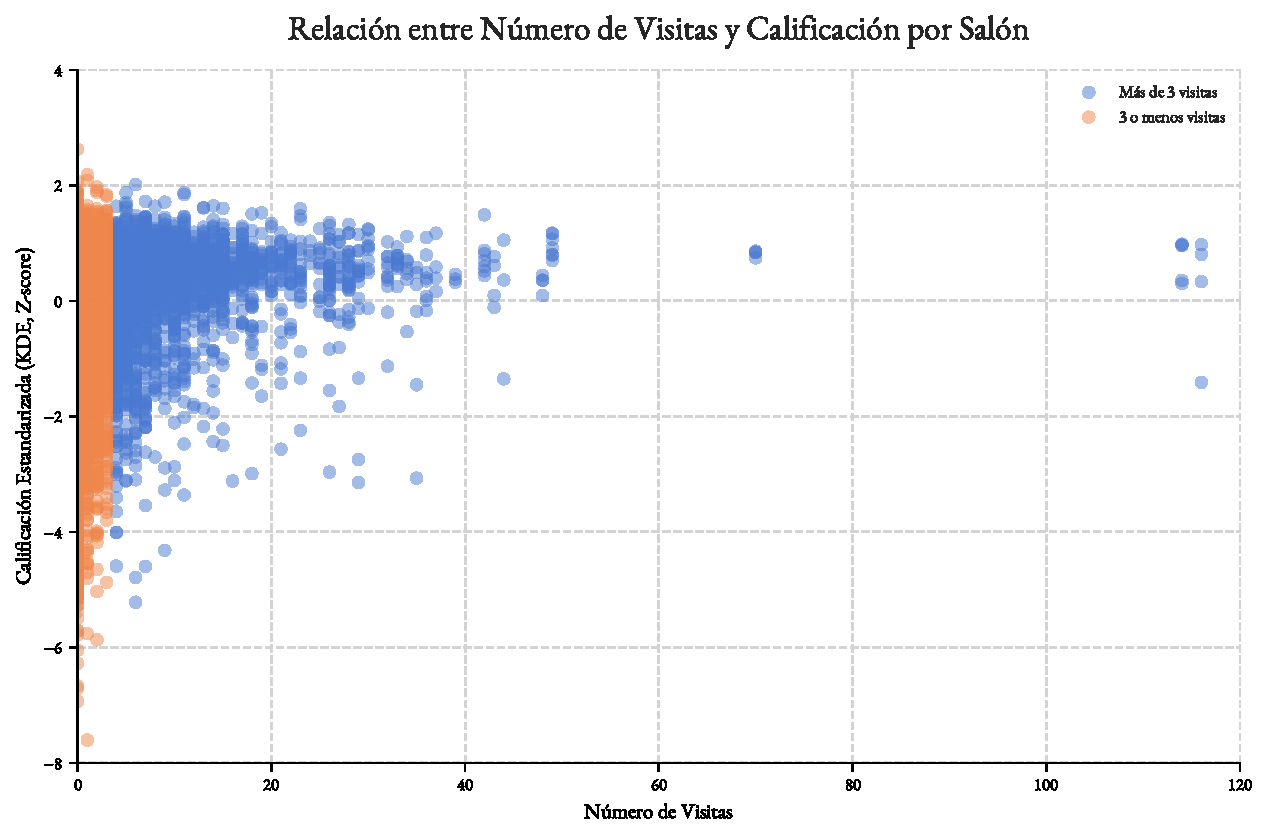
\includegraphics[width=0.7\textwidth,page=1]{07_00.pdf}
    \caption{PDF imported as image}
\end{figure}
\lipsum[1]

\subsection{Difference of means}
\lipsum[1]

\begin{figure}[h]
    \centering
    
\includegraphics[width=0.7\textwidth,page=1]{07_01.pdf}
    \caption{PDF imported as image}
\end{figure}
\lipsum[1]

\subsection{Confidence Intervals}
\lipsum[1]

\subsection{Robust tests}
\lipsum[1]

\begin{figure}[h]
    \centering
    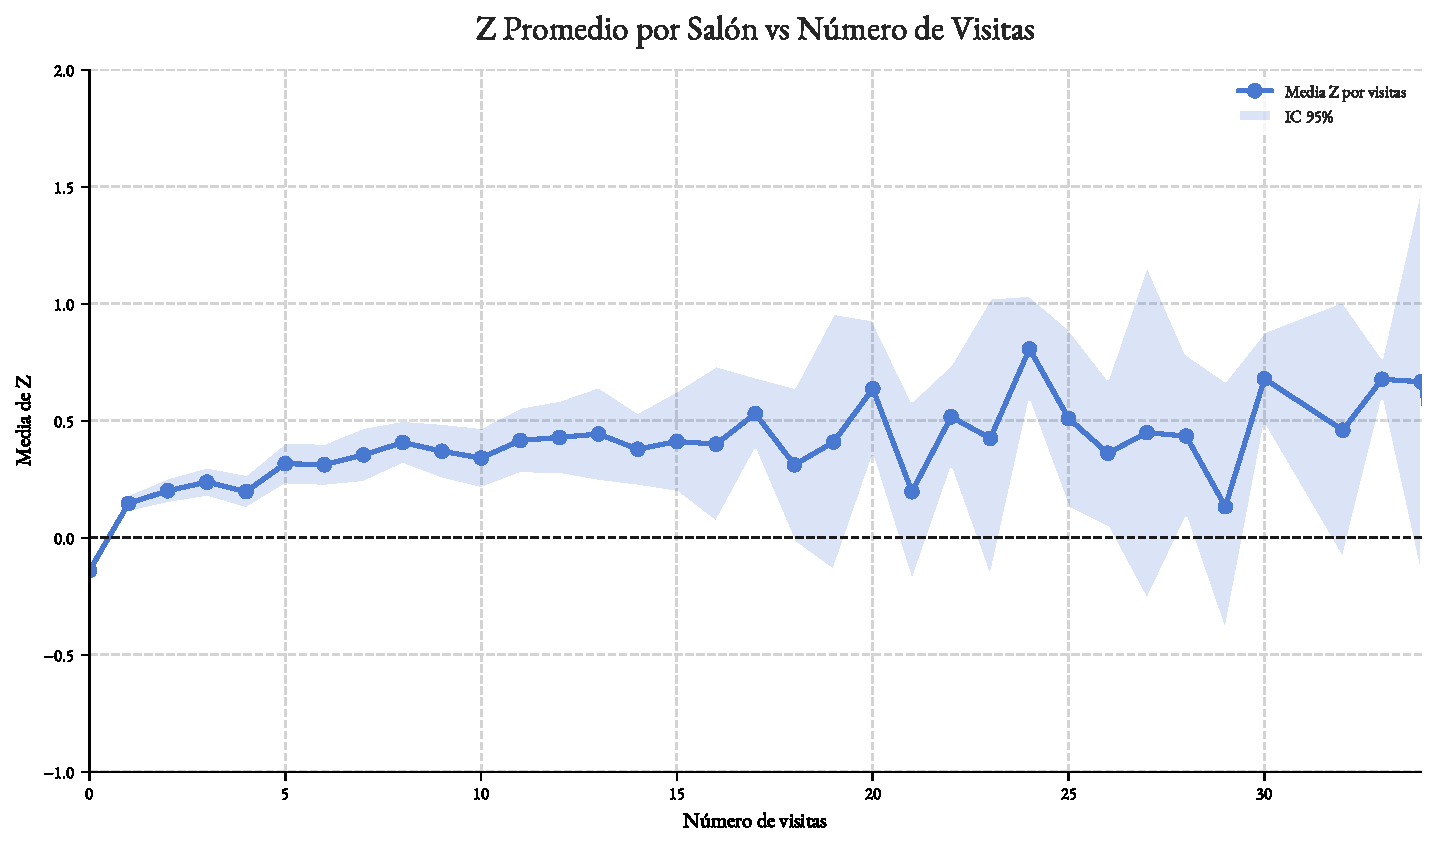
\includegraphics[width=0.7\textwidth,page=1]{09_01.pdf}
    \caption{PDF imported as image}
\end{figure}
\lipsum[1]

\subsection{Confidence intervals}
\lipsum[1]


\newpage
\section{Conclusions}

% Requires: \usepackage{amsmath, amssymb}

\subsection{Context and Variables}

The outcome variable is the standardized grade per student,
\texttt{MEAN\_IMPKDE\_Z}. For each classroom, raw grades were
standardized to a Z-score and missing values were imputed using
kernel density estimation (KDE). All analyses are therefore carried
out on a common standardized scale within classrooms.

Students were divided into two groups according to their cumulative
use of the CMAT (Mathematics Learning Center):
\begin{itemize}
  \item \textbf{Group A (frequent CMAT)}: students with more than three
        recorded visits to CMAT ($n_A = 1036$).
  \item \textbf{Group B (infrequent / non-CMAT)}: students with three
        or fewer recorded visits ($n_B = 9377$).
\end{itemize}

The goal is to quantify the association between frequent CMAT
attendance and standardized grades. Because the distribution of
standardized grades is non-normal and includes imputed values, the
primary analyses rely on robust nonparametric methods, complemented
by classical mean-based comparisons.

\subsection{Robust Nonparametric Comparison}

\subsubsection{Medians and Median Difference}

The sample medians are
\[
\operatorname{Median}_A = 0.422, \qquad
\operatorname{Median}_B = 0.185.
\]
Thus, a typical frequent CMAT student is about $0.42$ standard
deviations above the classroom mean, whereas a typical infrequent
or non-CMAT student is about $0.19$ standard deviations above the
classroom mean.

The difference in medians is
\[
\Delta_{\text{med}} = \operatorname{Median}_A - \operatorname{Median}_B
= 0.237.
\]
A nonparametric bootstrap with $B=8000$ resamples yields a 95\%
confidence interval for the median difference of
\[
\Delta_{\text{med}} \in [0.202,\; 0.284].
\]
This interval lies entirely above zero, indicating that a null
hypothesis of no difference in medians is not compatible with the
data.

Substantively, frequent CMAT students tend to lie roughly one
quarter of a standard deviation higher on standardized grades than
their peers.

\subsubsection{Permutation Test for the Median}

A two-sample permutation test was conducted for the median
difference. Under the null hypothesis that CMAT frequency has no
effect and that group labels (more than three vs.\ three or fewer
visits) are exchangeable, the observed statistic is
$\Delta_{\text{med}} = 0.237$.

Based on $5000$ random relabelings, the two-sided permutation
p-value is
\[
p_{\text{perm, median}} \approx 0.0004.
\]
Hence, if the null hypothesis were true, a median difference as
large as the one observed would occur in only about $0.04\%$ of
random permutations. This provides strong evidence that the two
groups differ in central tendency.

\subsubsection{Mann--Whitney U and Common-Language Effect Size}

The Mann--Whitney U test compares the distributions using rank
information. The test of equality of distributions yields
\[
p_{\text{MW}} = 3.224 \times 10^{-50},
\]
which is effectively zero at any conventional significance level.
Thus, the null hypothesis of identical distributions is strongly
rejected.

The associated common-language effect size (CL) is estimated as
\[
\text{CL} = 0.641,
\]
with a 95\% confidence interval of
\[
\text{CL} \in [0.625,\; 0.657].
\]
This quantity can be interpreted as the probability that a randomly
selected frequent CMAT student has a higher standardized grade than
a randomly selected infrequent/non-CMAT student, after taking the
more favorable direction. If the two groups were identical, CL
would equal $0.5$. The estimate of approximately $0.64$ with a
narrow confidence interval well above $0.5$ indicates a consistent
advantage for frequent CMAT attendees.

\subsubsection{Rank-Biserial Correlation}

The rank-biserial correlation derived from the Mann--Whitney test
is
\[
r_{\text{rb}} = 0.282,
\]
with 95\% confidence interval $[0.250,\; 0.313]$. This effect size
is correlation-like and ranges from $-1$ to $1$. Conventional
benchmarks in the behavioral sciences regard absolute values around
$0.1$ as small, $0.3$ as moderate, and $0.5$ or larger as large.
Thus, $r_{\text{rb}} \approx 0.28$ corresponds to a small-to-moderate
upward shift in the distribution of grades for frequent CMAT
students.

\subsubsection{Brunner--Munzel Test}

The Brunner--Munzel test is a rank-based method that is robust to
heteroscedasticity and differences in distributional shape between
groups. The two-sided test yields
\[
p_{\text{BM}} = 2.023 \times 10^{-57},
\]
again providing overwhelming evidence against the null hypothesis
of equal distributions. The agreement between Mann--Whitney and
Brunner--Munzel suggests that the main findings are not driven by
differences in variance or skewness alone.

\subsubsection{Cliff's Delta}

Cliff's delta is another nonparametric effect size summarizing
stochastic dominance:
\[
\delta = P(X>Y) - P(Y>X),
\]
where $X$ is a grade from the frequent CMAT group and $Y$ is a
grade from the infrequent/non-CMAT group. The estimate is
\[
\hat{\delta} = 0.283,
\]
with 95\% confidence interval
\[
\delta \in [0.234,\; 0.326].
\]
Thus, the probability that a frequent CMAT student outperforms an
infrequent/non-CMAT student exceeds the opposite probability by
approximately $28$ percentage points. As with $r_{\text{rb}}$, this
is typically interpreted as a small-to-moderate effect size.

\subsubsection{Mean-Based Comparison (t-Test and Cohen's \texorpdfstring{$d$}{d})}

To complement the robust analyses, a classical comparison of means
was performed. The sample means are
\[
\bar{x}_A = 0.34, \qquad \bar{x}_B = -0.08.
\]
The difference in means is therefore
\[
\bar{x}_A - \bar{x}_B = 0.41 \text{ Z-units}.
\]

A two-sample t-test (assuming equal or Welch-corrected variances)
produced a test statistic of
\[
t \approx 21.93,
\]
with approximately $n_A + n_B - 2 \approx 10{,}411$ degrees of
freedom. The associated p-value is much smaller than $10^{-10}$ (on
the order of $10^{-100}$), again indicating that the null hypothesis
of equal means is incompatible with the observed data.

From the reported $t$ and difference in means, the pooled standard
deviation can be reconstructed as $s_p \approx 0.57$. The standard
errors of the group means are then
\[
\text{SE}_A = \frac{s_p}{\sqrt{n_A}} \approx 0.0177, \qquad
\text{SE}_B = \frac{s_p}{\sqrt{n_B}} \approx 0.0059.
\]

Approximate 95\% confidence intervals are
\[
\bar{x}_A \in [0.31,\; 0.37], \qquad
\bar{x}_B \in [-0.092,\; -0.068],
\]
and for the mean difference
\[
\bar{x}_A - \bar{x}_B \in [0.37,\; 0.45].
\]
Thus, on average, frequent CMAT students are between $0.37$ and
$0.45$ standard deviations above infrequent/non-CMAT students on
the standardized scale.

The standardized mean difference (Cohen's $d$) is
\[
d = \frac{\bar{x}_A - \bar{x}_B}{s_p} \approx \frac{0.41}{0.57}
\approx 0.72.
\]
Using conventional benchmarks (0.2 small, 0.5 medium, 0.8 large),
this represents a medium-to-large effect, consistent with a
substantively meaningful difference in educational outcomes.

\subsection{Integrated Interpretation}

Taken together, the nonparametric and parametric analyses lead to a
coherent picture:
\begin{itemize}
  \item \textbf{Direction.} All measures---median difference, common-language
        effect size, rank-biserial correlation, Cliff's delta, and
        the difference in means---indicate that students who visit
        CMAT more than three times tend to achieve higher
        standardized grades than those who visit three or fewer
        times.
  \item \textbf{Magnitude.} In terms of central tendency, the median
        for frequent CMAT students is about $0.24$ standard
        deviations higher, and the mean is about $0.41$ standard
        deviations higher. In pairwise terms, frequent CMAT
        students are expected to outperform infrequent/non-CMAT
        students roughly $64\%$ of the time, with an excess win
        probability of about $28$ percentage points.
  \item \textbf{Statistical evidence.} All p-values from the Mann--Whitney,
        Brunner--Munzel, permutation, and t-tests are extremely
        small. The findings are not marginally significant; they
        represent very strong statistical evidence of association.
  \item \textbf{Robustness.} The conclusions are supported both by
        distribution-free methods (ranks, medians, Cliff's delta,
        bootstrap) and by classical mean-based inference, suggesting
        that the result is not an artifact of non-normality or
        heteroscedasticity.
\end{itemize}

In summary, frequent CMAT attendance is strongly and consistently
associated with improved standardized performance. As W.~Edwards
Deming is often paraphrased: \emph{``In God we trust; all others
must bring data.''} In this dataset, the data indicate a clear and
robust performance advantage for students who engage more
intensively with the CMAT.

\subsection{Limitations and Causal Interpretation}

Despite the strength of the association, these analyses are based
on observational data and do not, by themselves, establish a causal
effect of CMAT attendance on grades. Several caveats apply:

\begin{itemize}
  \item \textbf{Self-selection.} Students with higher prior ability,
        greater motivation, or other unobserved advantages may be
        more likely to use CMAT frequently. In that case, part of
        the observed effect reflects selection into CMAT rather
        than the impact of CMAT itself.
  \item \textbf{Unobserved confounding.} The standardization by
        classroom and KDE-based imputation control some aspects of
        the data-generating process, but not others, such as prior
        GPA, socioeconomic status, or access to private tutoring.
  \item \textbf{Imputation assumptions.} KDE-based imputation
        assumes that missingness mechanisms are not systematically
        different between groups. If missing grades are more likely
        in one group for reasons related to performance, the
        imputation may introduce bias.
\end{itemize}

For these reasons, the most defensible substantive claim is that
frequent CMAT attendance is \emph{strongly associated} with higher
standardized performance. Demonstrating that CMAT causes higher
grades would require additional causal design elements, such as
longitudinal models, matching or weighting on baseline covariates,
or experimental interventions.

\subsection{Concise Quantitative Summary}

The core quantitative results can be summarized as
\[
\boxed{
  \Delta_{\text{med}} \approx 0.24 \text{ Z-units (95\% CI [0.20, 0.28])},\quad
  \text{CL} \approx 0.64,\quad
  \delta \approx 0.28,\quad
  d \approx 0.72.
}
\]
Frequent CMAT users outperform infrequent or non-users with a
small-to-moderate but robust advantage in standardized grades.


\end{document}
